\chapter{MAC}

Con \textit{Message Authentication Code} si intende un blocco di dati che preso in input 
un messaggio ed una chiave segreta, restituisce un codice MAC; il destinatario, alla ricezione del 
messaggio e del MAC, farà la stessa procedura per vedere se i codici MAC coincidono.

\begin{figure}[H]
    \centering
    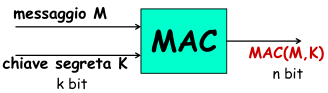
\includegraphics[width=0.7\linewidth]{chapters/chap06/images/mac.png}
\end{figure}

\noindent Viene usato per due scopi:
\begin{itemize}
    \item autenticità del messaggio 
    \item integrità del messaggio
\end{itemize}

\noindent MAC fornisce solo autenticità e integrità; se si vuole anche \textbf{condifenzialità},
si può cifrare prima o dopo con un'altra chiave (diversa da quella del MAC).

\begin{figure}[H]
    \centering
    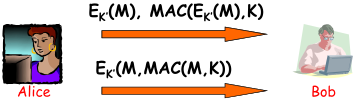
\includegraphics[width=0.8\linewidth]{chapters/chap06/images/conf.png}
\end{figure}

\newpage
\subsubsection{Proprietà}

\begin{itemize}
    \item \textbf{\textit{Easy computation:}} dato un messaggio $M$ e la chiave $k$, $MAC(M,k)$ è facile da calcolare 
    \item \textbf{\textit{Compression:}} output di lunghezza fissata
    \item \textbf{\textit{Computation-resistance:}} data una o più coppie $(m, f_k(m))$ non deve 
    essere possibile calcolarne altre; questa proprietà implica la \textit{key-non-recovery}, ma non 
    è vero il viceversa
    \item \textbf{\textit{Key-non-recovery:}} data una o più coppie $(m, f_k(m))$ deve essere impossibile ricavare 
    la chiave $k$
\end{itemize}

\subsubsection{Attacchi}

Si possono distinguere in base a:
\begin{itemize}
    \item Scopo dell'attacco:
    \begin{itemize}
        \item \textit{Total break:} determinare la chiave 
        \item \textit{Selective forgery:} dato $m$, determinare $y$ tale che $y=MAC(m, k)$
        \item \textit{Existential forgery:} determinare una coppia $(y,m)$ tale che $y=MAC(m, k)$
    \end{itemize}
    \item Tipo di attacco:
    \begin{itemize}
        \item \textit{Known message} (conosce una lista di messaggi e relativi MAC)
        \item \textit{Chosen message} (sceglie i messaggi e può calcolare i relativi MAC)
        \item \textit{Adaptive chosen message} (come il precedente ma le scelte dipendono dalle risposte precedenti)
    \end{itemize}
\end{itemize}

\noindent È ovviamente possible fare anche attacchi di forza bruta, motivo per cui è consigliabile 
avere una chiave di almeno 128 bit.

\newpage
\section{HMAC}

È una funzione che permette di calcolare un MAC tramite una funzione di hash qualsiasi e una 
chiave segreta; l'indipendenza dalla funzione di hash precisa è dovuta alla necessità di 
doverla sostituire nel caso in cui non sia più sicura.

\begin{itemize}
    \item Data una funzione di hash $h$, un messaggio $m$, e una chiave $k$, hmac opera utilizzando 
    blocchi di $b$ byte
    \begin{itemize}
        \item nel caso la chiave sia più lunga di $b$ byte, le si applica la funzione di hash in modo 
        da ottenerla lunga $b$ byte 
        \item nel caso la chiave sia più corta, si aggiunge del padding 
    \end{itemize}
    \item vengono definite due stringhe:
    \begin{itemize}
        \item $ipad:$ byte 0x36 ripetuto $\frac{b}{8}$ volte
        \item $opad:$ byte 0x5c ripetuto $\frac{b}{8}$ volte
    \end{itemize}
    \item la funzione prende $m$ e $k$ producendo il MAC secondo la formula 
    \begin{center}
        $h(k \oplus opad$  $||$ $h(k \oplus ipad$ $||$ $m))$
    \end{center}
\end{itemize}
\noindent 

\noindent In generale, HMAC è sicuro se la funzione di hash usata è sicura.


